\documentclass[11pt]{uiobrev}
\usepackage[utf8]{inputenc}
\usepackage[T1]{fontenc}
\usepackage[portuguese]{babel}
\usepackage{tgtermes, xurl, textpos, graphicx, geometry}
\usepackage{enumitem}
\usepackage{fancyhdr}
\usepackage{ragged2e}
\documentclass{article}
\usepackage[utf8]{inputenc}
\usepackage[T1]{fontenc}
\usepackage{listings}
\usepackage{courier}

\lstset{
  language=Java,
  basicstyle=\ttfamily\small,
  keywordstyle=\color{blue}\bfseries,
  commentstyle=\color{gray},
  stringstyle=\color{red},
  numbers=left,
  numberstyle=\tiny,
  stepnumber=1,
  numbersep=5pt,
  showspaces=false,
  showstringspaces=false,
  frame=single,
  tabsize=4,
  breaklines=true,
  breakatwhitespace=false,
  escapeinside={(*@}{@*)} % Permite comentários personalizados
}

\geometry{a4paper, vmargin=3.5cm, hmargin=2.5cm}
\name{Arthur Dantas}
\date{17 de Novembro de 2024}


\pagestyle{fancy}
\fancyhf{} 
\fancyhead[R]{\thepage}
\renewcommand{\headrulewidth}{0pt}

\begin{document}

\begin{letter}{\\Arthur Silva Dantas \\ Graziela Santos de Araújo}

    \opening{Relatório: Trabalho Prático - Linguagem de Programação Orientada a Objetos}

    Olá,

    Este relatório destina-se ao trabalho prático da disciplina de Linguagem de Programação Orientada a Objetos, onde o projeto simula um jogo de RPG utilizando os princípios de Orientação a Objetos e aplicando o conteúdo abordado ao longo da disciplina.

    \bigskip
    Para obter mais informações sobre o código completo e consultar uma parte adicional da documentação, o projeto está disponível no GitHub. 
    \\ Disponível em: \url{https://github.com/Arthur-SD15/LPOO-RolePlayingGame}.

    \closing{Atenciosamente,}
\thispagestyle{empty} 
\end{letter}

\newpage

\begin{center}
    \Large \textbf{Sumário}
\end{center}
\vspace{1cm}

\begin{enumerate}
    \item \textbf{Projeto Geral} \dotfill \textbf{1}
    \item \textbf{Organização Geral} \dotfill \textbf{1}
    \item \textbf{Organização Detalhada} \dotfill \textbf{2}
        \begin{enumerate}[label*=\arabic*.] 
            \item \textbf{Personagem.java} \dotfill \textbf{2}
            \item \textbf{Arma.java} \dotfill \textbf{5}
            \item \textbf{Mago.java} \dotfill \textbf{5}
            \item \textbf{Paladino.java} \dotfill \textbf{6}
            \item \textbf{Clerigo.java} \dotfill \textbf{7}
            \item \textbf{ArmaMago.java} \dotfill \textbf{7}
            \item \textbf{ArmaPaladino.java} \dotfill \textbf{8}
            \item \textbf{ArmaClerigo.java} \dotfill \textbf{8}
            \item \textbf{Transmutação.java} \dotfill \textbf{9}
            \item \textbf{Psikappa.java} \dotfill \textbf{10}
            \item \textbf{Espada.java} \dotfill \textbf{10}
            \item \textbf{Lança.java} \dotfill \textbf{11}
            \item \textbf{Martelo.java} \dotfill \textbf{12}
            \item \textbf{Maça.java} \dotfill \textbf{12}
            \item \textbf{Main.java} \dotfill \textbf{13}
        \end{enumerate}
    \item \textbf{Dificuldades Encontradas} \dotfill \textbf{17}
    \item \textbf{Soluções} \dotfill \textbf{18}
\end{enumerate}
\thispagestyle{empty}

\newpage

\setcounter{page}{1}

\noindent
\Large \textbf{1. Projeto Geral}

\justifying
O projeto, de maneira geral, consiste em códigos e documentações de um trabalho prático da disciplina de Linguagem de Programação Orientada a Objetos, desenvolvido na Universidade Federal de Mato Grosso do Sul. Ele simula um Role Playing Game (RPG), um jogo via linha de comando, no qual foram aplicados os fundamentos da Orientação a Objetos utilizando a linguagem Java. O código contém comentários explicativos sobre as operações realizadas e inclui um relatório, onde se lê, tal documento, o objetivo é documentar o projeto com maiores detalhes.

\vspace{1.5cm}
\Large \textbf{2. Organização Geral}

\justifying
Nesta seção, começamos a detalhar e explorar a estrutura do projeto e, consequentemente, do código. No entanto, a análise detalhada do código ficará para a seção posterior. O objetivo desta seção é abordar a estrutura e alguns conceitos teóricos, a fim de facilitar a compreensão da próxima seção.

Antes de tudo, o projeto segue rigorosamente os princípios da Orientação a Objetos, contendo 15 arquivos .java com \textbf{classes abstratas, concretas e hierarquias de herança}. Antes que eu me esqueça, acho importante destacar que, de maneira geral, todos os atributos são privados. Durante a minha implementação o código em si, não foi necessário, e consequentemente não foi feito uso de sobrecarga, nem mesmo nos construtores. Além disso, não foi utilizado o método @Override para sobrescrita. De maneira geral, foram trabalhados, em especial, o polimorfismo, o encapsulamento e a abstração.

Como apoio, foi utilizado um Diagrama de Classes da UML (Unified Modeling Language), que havia sido disponibilizado pela professora e serviu como base ao longo do desenvolvimento.

Durante o projeto, os conceitos de Orientação a Objetos são evidentes, permitindo identificar relações de \textbf{herança}, como a herança da classe Personagem para as classes Clérigo, Paladino e Mago, que são suas subclasses. Vale destacar, que a herança tem por objetivo a reutilização de código permitindo que as subclasses herdem atributos e métodos das classes pai, além de poder adicionar ou modificar funcionalidades específicas.

Uma observação é que não existe apenas essa herança dentro do projeto. Assim como também não existe apenas a \textbf{classe abstrata} Personagem, que tem por objetivo servir como molde para outras \textbf{classes concretas}.

\vspace{1.5cm}
\Large \textbf{3. Organização Detalhada}

\justifying
Confira a organização detalhada, com base em alguns conceitos teóricos e entrando a fundo em cada código implementado.

\vspace{0.5cm}
\Large \textbf{3.1. Personagem.java}

Neste arquivo, temos a classe abstrata Personagem, que serve como classe pai para todas as outras classes de personagens e é utilizada como molde.

A classe contém atributos privados relacionados ao personagem, acompanhados de seus respectivos métodos getters e setters. Também inclui o construtor da classe, o método printStatus, que imprime o status do personagem e o método atacar baseado em diversas condições, que será detalhado na seção 4, ao tratar das dificuldades encontradas. O método calculaDano, que calcula o dano causado pelo personagem; o receberDano, que calcula o dano recebido pelo personagem e por fim o estaMorto, que verifica se o personagem está morto.

Código completo, com comentários: 

\begin{lstlisting}[language=Java, caption={Classe abstrata \texttt{Personagem}}]
/*
 * Importamos as classes necessarias: BigDecimal e RoundingMode.
 * BigDecimal: permite trabalhar com numeros decimais com precisao.
 * RoundingMode: permite trabalhar com arredondamento de numeros decimais.
*/
import java.math.BigDecimal;
import java.math.RoundingMode;

// Classe abstrata Personagem.
public abstract class Personagem {
    // Atributos da classe Personagem.
    private String nomeTipo;
    private double saude;
    private double forca;
    private double destreza;
    private Arma arma;

    // Construtor da classe Personagem.
    public Personagem(String nomeTipo, double saude, double forca, double destreza, Arma arma) {
        this.nomeTipo = nomeTipo;
        this.saude = saude;
        this.forca = forca;
        this.destreza = destreza;
        this.arma = arma;
    }

    // Metodos getters e setters da classe Personagem.
    public String getNomeTipo() { return this.nomeTipo; }
    public double getSaude() { return this.saude; }
    public double getForca() { return this.forca; }
    public double getDestreza() { return this.destreza; }
    public Arma getArma() { return this.arma; }
    public void setNomeTipo(String nomeTipo) { this.nomeTipo = nomeTipo; }
    public void setSaude(double saude) { this.saude = saude; }
    public void setForca(double forca) { this.forca = forca; }
    public void setDestreza(double destreza) { this.destreza = destreza; }
    public void setArma(Arma arma) { this.arma = arma; }

    /*
     * Metodo printStatus que imprime o status do personagem.
     * Utiliza getters para acessar os atributos privados.
    */
    public void printStatus() {
        if (estaMorto()) {
            System.out.printf(getNomeTipo() + " [Morto, Forca: %.1f, Destreza: %.1f, %s]\n",
                getForca(), getDestreza(), getArma().getNome());
        } else {
            System.out.printf(getNomeTipo() + " [Saude: %.1f, Forca: %.1f, Destreza: %.1f, %s]\n",
                getSaude(), getForca(), getDestreza(), getArma().getNome());
        }
    }

    /*
     * Metodo atacar que realiza um ataque a outro personagem.
     * Possui condicoes baseadas na destreza dos personagens.
    */
    public void atacar(Personagem b) {
        if (estaMorto()) {
            System.out.println("O " + getNomeTipo() + " nao pode atacar, pois esta morto.");
            return;
        } else {
            System.out.println("O " + getNomeTipo() + " ataca o " + b.getNomeTipo() + " com " + getArma().getNome() + ".");
        }

        if (b.estaMorto()) {
            System.out.println("Pare! O " + b.getNomeTipo() + " ja esta morto!");
            return;
        }

        if (getDestreza() > b.getDestreza()) {
            double auxDanoSofrido = calculaDano();
            System.out.printf("O ataque foi efetivo com %.1f pontos de dano!\n", auxDanoSofrido);
            b.receberDano(auxDanoSofrido);
        } else if (getDestreza() < b.getDestreza()) {
            double auxDanoSofrido = b.calculaDano();
            System.out.printf("O ataque foi inefetivo e revidado com %.1f pontos de dano!\n", auxDanoSofrido);
            receberDano(auxDanoSofrido);
        } else {
            System.out.println("O ataque foi defendido, ninguem se machucou!");
        }
    }

    /*
     * Metodo calculaDano que calcula o dano causado.
     * Utiliza BigDecimal para precisao no calculo.
    */
    private double calculaDano() {
        BigDecimal dano = new BigDecimal(getForca() * getArma().getModDano());
        return dano.setScale(1, RoundingMode.HALF_UP).doubleValue();
    }

    /*
     * Metodo receberDano que aplica o dano recebido ao personagem.
    */
    private double receberDano(double pontosDano) {
        this.saude -= pontosDano;
        return this.saude;
    }

    /*
     * Metodo estaMorto que verifica se o personagem esta morto.
     * Retorna true se a saude for menor que 1, caso contrario, false.
    */
    private boolean estaMorto() {
        return getSaude() < 1;
    }
}
\end{lstlisting}

\newpage
\Large \textbf{3.2. Arma.java}

A classe Arma possui semelhanças com a classe Personagem, sendo uma classe abstrata que serve como classe molde para outras classes. Ela contém dois atributos privados, que são acessados por meio de métodos getters. Além disso, a classe possui um construtor que recebe dois parâmetros: o nome da arma e o modificador.

Código completo, com comentários: 

\begin{lstlisting}[language=Java, caption={Classe Abstrata Arma}]
// Classe abstrata Arma.
public abstract class Arma{
    // Atributos da classe Arma.
    private String nome;
    private double modDano;

    // Construtor da classe Arma.
    public Arma(String nome, double modDano){
        this.nome = nome;
        this.modDano = modDano;
    }

    // Metodos getters da classe Arma.
    public String getNome(){
        return this.nome;
    }

    public double getModDano(){
        return this.modDano;
    }
}
\end{lstlisting}


\vspace{0.5cm}
\Large \textbf{3.3. Mago.java}

Este arquivo é responsável por criar a classe Mago, que é uma subclasse de Personagem. Dentro dessa classe, temos o construtor da classe Mago, que recebe os atributos do personagem e a arma. O construtor da superclasse é utilizado para inicializar os atributos do personagem.

Código completo, com comentários: 

\newpage
\begin{lstlisting}[language=Java, caption={Classe Mago, subclasse de Personagem}]
/*
 * Criamos a classe Mago que e uma subclasse de Personagem, herdando os atributos e metodos de personagem.
 * Essa classe e responsavel por criar um personagem do tipo Mago.
 * Dentro dessa classe, temos o construtor da classe Mago que recebe os valores de saude, forca, destreza e a arma.
 * Utilizamos o construtor da superclasse para inicializar os atributos de personagem.
*/
public class Mago extends Personagem{
    public Mago(double saude, double forca, double destreza, ArmaMago arma){
        super("Mago", saude, forca, destreza, arma);
    }
}
\end{lstlisting}

\vspace{0.5cm}
\Large \textbf{3.4. Paladino.java}

Este arquivo é responsável por criar a classe Paladino, que é uma subclasse de Personagem. Dentro dessa classe, temos o construtor da classe Paladino, que recebe os atributos do personagem e a arma. O construtor da superclasse é utilizado para inicializar os atributos do personagem.

Código completo, com comentários: 

\begin{lstlisting}[language=Java, caption={Classe Paladino, subclasse de Personagem}]
/*
 * Criamos a classe Paladino que e uma subclasse de Personagem, herdando os atributos e metodos de personagem.
 * Essa classe e responsavel por criar um personagem do tipo Paladino.
 * Dentro dessa classe, temos o construtor da classe Paladino que recebe os valores de saude, forca, destreza e a arma.
 * Utilizamos o construtor da superclasse para inicializar os atributos de personagem.
*/
public class Paladino extends Personagem {
    public Paladino(double saude, double forca, double destreza, ArmaPaladino arma) {
        super("Paladino", saude, forca, destreza, arma);
    }
}
\end{lstlisting}

\newpage
\Large \textbf{3.5. Clerigo.java}

Este arquivo é responsável por criar a classe Clérigo, que é uma subclasse de Personagem. Dentro dessa classe, temos o construtor da classe Clérigo, que recebe os atributos do personagem e a arma. O construtor da superclasse é utilizado para inicializar os atributos do personagem.

Código completo, com comentários: 

\begin{lstlisting}[language=Java, caption={Classe Clerigo, subclasse de Personagem}]
/*
 * Criamos a classe Clerigo que e uma subclasse de Personagem, herdando os atributos e metodos de personagem.
 * Essa classe e responsavel por criar um personagem do tipo Clerigo.
 * Dentro dessa classe, temos o construtor da classe Clerigo que recebe os valores de saude, forca, destreza e a arma.
 * Utilizamos o construtor da superclasse para inicializar os atributos de personagem.
*/
public class Clerigo extends Personagem{
    public Clerigo(double saude, double forca, double destreza, ArmaClerigo arma){
        super("Clerigo", saude, forca, destreza, arma);
    }
}
\end{lstlisting}

\vspace{0.5cm}
\Large \textbf{3.6. ArmaMago.java}

Este arquivo é responsável por criar a classe ArmaMago, que é uma subclasse de Arma. Dentro dessa classe, temos o construtor da classe ArmaMago, que recebe os atributos da arma. O construtor da superclasse é utilizado para inicializar os atributos da arma.

Código completo, com comentários: 

\begin{lstlisting}[language=Java, caption={Classe ArmaMago, subclasse de Arma}]
/*
 * Criamos uma classe abstrata ArmaMago que e uma subclasse de Arma, herdando os atributos de arma. 
 * Essa classe e responsavel por criar uma ArmaMago do tipo Arma.
 * Dentro dessa classe, temos o construtor da classe ArmaMago que recebe o nome e o modificador de dano.
 * Utilizamos o construtor da superclasse para inicializar os atributos de arma.
*/
public abstract class ArmaMago extends Arma{
    public ArmaMago(String nome, double modDano){
        super(nome, modDano);
    }
}
\end{lstlisting}

\vspace{0.5cm}
\Large \textbf{3.7. ArmaPaladino.java}

Este arquivo é responsável por criar a classe ArmaPaladino, que é uma subclasse de Arma. Dentro dessa classe, temos o construtor da classe ArmaPaladino, que recebe os atributos da arma. O construtor da superclasse é utilizado para inicializar os atributos da arma.

Código completo, com comentários: 

\begin{lstlisting}[language=Java, caption={Classe ArmaPaladino, subclasse de Arma}]
/*
 * Criamos uma classe abstrata ArmaPaladino que e uma subclasse de Arma, herdando os atributos de arma. 
 * Essa classe e responsavel por criar uma ArmaPaladino do tipo Arma.
 * Dentro dessa classe, temos o construtor da classe ArmaPaladino que recebe o nome e o modificador de dano.
 * Utilizamos o construtor da superclasse para inicializar os atributos de arma.
*/
public abstract class ArmaPaladino extends Arma{
    public ArmaPaladino(String nome, double modDano){
        super(nome, modDano);
    }
}
\end{lstlisting}

\vspace{0.5cm}
\Large \textbf{3.8. ArmaClerigo.java}

Este arquivo é responsável por criar a classe ArmaClerigo, que é uma subclasse de Arma. Dentro dessa classe, temos o construtor da classe ArmaClerigo, que recebe os atributos da arma. O construtor da superclasse é utilizado para inicializar os atributos da arma.

Código completo, com comentários: 

\newpage
\begin{lstlisting}[language=Java, caption={Classe ArmaClerigo, subclasse de Arma}]
/*
 * Criamos uma classe abstrata ArmaClerigo que e uma subclasse de Arma, herdando os atributos de arma. 
 * Essa classe e responsavel por criar uma ArmaClerigo do tipo Arma.
 * Dentro dessa classe, temos o construtor da classe ArmaClerigo que recebe o nome e o modificador de dano.
 * Utilizamos o construtor da superclasse para inicializar os atributos de arma.
*/
public abstract class ArmaClerigo extends Arma{
    public ArmaClerigo(String nome, double modDano){
        super(nome, modDano);
    }
}
\end{lstlisting}

\vspace{0.5cm}
\Large \textbf{3.9. Transmutação.java}

Este arquivo é responsável por criar a classe Transmutacao, que é uma subclasse de ArmaMago. Dentro dessa classe, temos o construtor da classe Transmutacao, que recebe os atributos da arma, como o nome e o modificador de dano. O nome da arma é "Magia da Transmutação" e o modificador de dano é 0.25. O construtor da superclasse ArmaMago é utilizado para inicializar esses atributos.

Código completo, com comentários: 

\begin{lstlisting}[language=Java, caption={Classe Transmutacao, subclasse de ArmaMago}]
/*
 *  Criamos a classe Transmutacao que e uma subclasse de ArmaMago, herdando os atributos de ArmaMago.
 *  Essa classe e responsavel por criar uma Arma de Mago do tipo Transmutacao.
 *  Dentro dessa classe, temos o construtor da classe Transmutacao que recebe o nome e o dano da arma.
 *  Utilizamos o construtor da superclasse para inicializar os atributos de ArmaMago.
*/
public class Transmutacao extends ArmaMago {
    public Transmutacao() {
        super("Magia da Transmutacao", 0.25);
    }
}
\end{lstlisting}

\newpage
\Large \textbf{3.10. Psikappa.java}

Este arquivo é responsável por criar a classe Psikappa, que é uma subclasse de ArmaMago. Dentro dessa classe, temos o construtor da classe Psikappa, que recebe os atributos da arma, como o nome e o modificador de dano. O nome da arma é "Psi-kappa" e o modificador de dano é 0.5. O construtor da superclasse ArmaMago é utilizado para inicializar esses atributos.

Código completo, com comentários: 

\begin{lstlisting}[language=Java, caption={Classe Psikappa, subclasse de ArmaMago}]
/*
 *  Criamos a classe Psikappa que e uma subclasse de ArmaMago, herdando os atributos de ArmaMago.
 *  Essa classe e responsavel por criar uma Arma de Mago do tipo Psikappa.
 *  Dentro dessa classe, temos o construtor da classe Psikappa que recebe o nome e o dano da arma.
 *  Utilizamos o construtor da superclasse para inicializar os atributos de ArmaMago.
*/
public class Psikappa extends ArmaMago {
    public Psikappa() {
        super("Psi-kappa", 0.5);
    }
}
\end{lstlisting}

\vspace{0.5cm}
\Large \textbf{3.11. Espada.java}

Este arquivo é responsável por criar a classe Espada, que é uma subclasse de ArmaPaladino. Dentro dessa classe, temos o construtor da classe Espada, que recebe os atributos da arma, como o nome e o modificador de dano. O nome da arma é "Espada" e o modificador de dano é 0.3. O construtor da superclasse ArmaPaladino é utilizado para inicializar esses atributos.

Código completo, com comentários: 

\begin{lstlisting}[language=Java, caption={Classe Espada, subclasse de ArmaPaladino}]
/*
 *  Criamos a classe Espada que e uma subclasse de ArmaPaladino, herdando os atributos de ArmaPaladino.
 *  Essa classe e responsavel por criar uma Arma de Paladino do tipo Espada.
 *  Dentro dessa classe, temos o construtor da classe Espada que recebe o nome e o dano da arma.
 *  Utilizamos o construtor da superclasse para inicializar os atributos de ArmaPaladino.
*/
public class Espada extends ArmaPaladino {
    public Espada() {
        super("Espada", 0.3);
    }
}
\end{lstlisting}

\vspace{0.5cm}
\Large \textbf{3.12. Lança.java}

Este arquivo é responsável por criar a classe Lança, que é uma subclasse de ArmaPaladino. Dentro dessa classe, temos o construtor da classe Lança, que recebe os atributos da arma, como o nome e o modificador de dano. O nome da arma é "Lança" e o modificador de dano é 0.5. O construtor da superclasse ArmaPaladino é utilizado para inicializar esses atributos.

Código completo, com comentários: 

\begin{lstlisting}[language=Java, caption={Classe Lanca, subclasse de ArmaPaladino}]
/*
 *  Criamos a classe Lanca que e uma subclasse de ArmaPaladino, herdando os atributos de ArmaPaladino.
 *  Essa classe e responsavel por criar uma Arma de Paladino do tipo Lanca.
 *  Dentro dessa classe, temos o construtor da classe Lanca que recebe o nome e o dano da arma.
 *  Utilizamos o construtor da superclasse para inicializar os atributos de ArmaPaladino.
*/
public class Lanca extends ArmaPaladino {
    public Lanca() {
        super("Lanca", 0.5);
    }
}
\end{lstlisting}

\newpage
\Large \textbf{3.13. Martelo.java}

Este arquivo é responsável por criar a classe Martelo, que é uma subclasse de ArmaClerigo. Dentro dessa classe, temos o construtor da classe Martelo, que recebe os atributos da arma, como o nome e o modificador de dano. O nome da arma é "Martelo" e o modificador de dano é 0.6. O construtor da superclasse ArmaClerigo é utilizado para inicializar esses atributos.

Código completo, com comentários: 

\begin{lstlisting}[language=Java, caption={Classe Martelo, subclasse de ArmaClerigo}]
/*
 *  Criamos a classe Martelo que e uma subclasse de ArmaClerigo, herdando os atributos de ArmaClerigo.
 *  Essa classe e responsavel por criar uma Arma de Clerigo do tipo Martelo.
 *  Dentro dessa classe, temos o construtor da classe Martelo que recebe o nome e o dano da arma.
 *  Utilizamos o construtor da superclasse para inicializar os atributos de ArmaClerigo.
*/
public class Martelo extends ArmaClerigo {
    public Martelo(){
        super("Martelo", 0.6);
    }
}
\end{lstlisting}

\vspace{0.5cm}
\Large \textbf{3.14. Maça.java}

Este arquivo é responsável por criar a classe Maca, que é uma subclasse de ArmaClerigo. Dentro dessa classe, temos o construtor da classe Maca, que recebe os atributos da arma, como o nome e o modificador de dano. O nome da arma é "Maça" e o modificador de dano é 0.4. O construtor da superclasse ArmaClerigo é utilizado para inicializar esses atributos.

Código completo, com comentários: 

\newpage
\begin{lstlisting}[language=Java, caption={Classe Maça, subclasse de ArmaClerigo}]
/*
 *  Criamos a classe Maca que e uma subclasse de ArmaClerigo, herdando os atributos de ArmaClerigo.
 *  Essa classe e responsavel por criar uma Arma de Clerigo do tipo Maca.
 *  Dentro dessa classe, temos o construtor da classe Maca que recebe o nome e o dano da arma.
 *  Utilizamos o construtor da superclasse para inicializar os atributos de ArmaClerigo.
*/
public class Maca extends ArmaClerigo {
    public Maca(){
        super("Maca", 0.4);
    }
}
\end{lstlisting}

\vspace{0.5cm}
\Large \textbf{3.15. Main.java}

A classe Main é a classe principal do programa, onde o fluxo do programa é executado. No método main, inicialmente, diante de um problema, defini que o padrão de formatação de números decimais seja o americano, já que o padrão brasileiro utiliza vírgulas como separadores decimais, enquanto o americano utiliza pontos.

Em seguida, é criado um vetor de personagens com tamanho 2, pois o RPG será jogado com dois personagens: o atacante e o defensor. Dentro de um laço de repetição, iremos percorrer o vetor de personagens, e lemos o número do personagem e, em seguida, seus atributos. De acordo com os números inseridos para o personagem e a arma, primeiro a arma é instanciada e, em seguida, o personagem.

\begin{lstlisting}[language=Java, caption={Instanciação da Arma e do Personagem}]
case 1:
    ArmaMago armaMago;
    switch (numeroArma) {
        case 1:
            armaMago = new Transmutacao(); // A arma do mago e instanciada aqui com base no numero fornecido.
            break;
        case 2:
            armaMago = new Psikappa(); // Outra opcao de instancia para a arma do mago.
            break;
        default:
            throw new IllegalArgumentException("Arma inválida para Mago.");
    }
    personagens[i] = new Mago(numeroSaude, numeroForca, numeroDestreza, armaMago); // O personagem Mago é instanciado aqui com os atributos e a arma escolhida.
    break;
\end{lstlisting}

Após essa etapa, a batalha é iniciada. A batalha só é interrompida quando o número do personagem atacante ou do defensor for 0. Dentro do laço de repetição, são lidos os números dos personagens atacante e defensor, e então é realizado o ataque do personagem atacante contra o personagem defensor.

\begin{lstlisting}[language=Java, caption={While da Batalha}]
while (true) {
    // Le o numero do personagem atacante.
    int ataque = sc.nextInt();
    // Le o numero do personagem defensor.
    int defesa = sc.nextInt();

    // Caso o numero do personagem atacante ou defensor seja 0, o laço e interrompido.
    if (ataque == 0 || defesa == 0) {
        break;
    }

    /*
     * Dentro de [] utilizamos o -1, pois o vetor comeca em 0 
     * e o numero do personagem começa em 1. 
    */
    // Realizamos o ataque do personagem atacante no personagem defensor.
    personagens[ataque - 1].atacar(personagens[defesa - 1]);
    // Imprimimos o status do atacante.
    personagens[ataque - 1].printStatus();
    // Imprimimos o status do defensor.
    personagens[defesa - 1].printStatus();
}
\end{lstlisting}

    Código completo, com comentários: 

\begin{lstlisting}[language=Java, caption={Codigo Principal do Programa}]
/*
 * Importamos as classes necessarias, sendo elas: Locale e Scanner.
 * Locale: classe que permite a formatacao de numeros decimais, o padrao do Brasileiro e diferente do padrao Americano. O padrao brasileiro utiliza virgula como separador de casas decimais, enquanto o padrao americano utiliza ponto.
 * Scanner: classe que permite a leitura de dados.
*/
import java.util.Locale;
import java.util.Scanner;

// Classe Main que contem o metodo main, que e o metodo principal por executar o programa.
public class Main {
    // Metodo main que e o metodo principal por executar o programa.
    public static void main(String[] args) {
        // Define o padrao de formatacao de numeros decimais para o padrao americano.
        Locale.setDefault(Locale.US);

        // Cria um objeto sc da classe Scanner que permite a leitura de dados.
        Scanner sc = new Scanner(System.in);
        // Cria um vetor de personagens com tamanho 2, ja que nosso RPG sera de dois personagens.
        Personagem[] personagens = new Personagem[2];

        // Laco de repeticao para ler os dados dos personagens.
        for (int i = 0; i < 2; i++) {
            // Le o numero do personagem (1: Mago, 2: Paladino, 3: Clerigo).
            int numeroPersonagem = sc.nextInt();
            // Le os numeros de saude, forca, destreza.
            double numeroSaude = sc.nextDouble();
            double numeroForca = sc.nextDouble();
            double numeroDestreza = sc.nextDouble();
            // Le o numero da arma (Cada arma tem numero 1 e 2, mas varia entre os personagens).
            int numeroArma = sc.nextInt();

            /*
             * Verificamos o numero do personagem. De acordo com esse numero, ele entrara em um dos casos. Caso o numero seja diferente de 1, 2 ou 3 uma excecao sera lancada.
             * Todos os casos tem a mesma estrutura, mudando apenas a arma de acordo com o personagem. Segue a estrutura:
             * - De acordo com o numero do personagem, criamos inicialmente uma variavel do tipo da arma do personagem.
             * - Verificamos o numero da arma. De acordo com esse numero, instanciamos a arma do personagem. Caso o numero seja diferente de 1 ou 2, uma excecao sera lancada.
             * - Instanciamos o personagem, de acordo com o numero do personagem, passando os valores de saude, forca, destreza e a arma.
             * - Apos instanciarmos o personagem, ele e adicionado no vetor de personagens.
            */
            switch (numeroPersonagem) {
                case 1:
                    ArmaMago armaMago;
                    switch (numeroArma) {
                        case 1:
                            armaMago = new Transmutacao();
                            break;
                        case 2:
                            armaMago = new Psikappa();
                            break;
                        default:
                            throw new IllegalArgumentException("Arma invalida para Mago.");
                    }
                    personagens[i] = new Mago(numeroSaude, numeroForca, numeroDestreza, armaMago);
                    break;

                case 2:
                    ArmaPaladino armaPaladino;
                    switch (numeroArma) {
                        case 1:
                            armaPaladino = new Espada();
                            break;
                        case 2:
                            armaPaladino = new Lanca();
                            break;
                        default:
                            throw new IllegalArgumentException("Arma invalida para Paladino.");
                    }
                    personagens[i] = new Paladino(numeroSaude, numeroForca, numeroDestreza, armaPaladino);
                    break;

                case 3:
                    ArmaClerigo armaClerigo;
                    switch (numeroArma) {
                        case 1:
                            armaClerigo = new Martelo();
                            break;
                        case 2:
                            armaClerigo = new Maca();
                            break;
                        default:
                            throw new IllegalArgumentException("Arma invalida para Clerigo.");
                    }
                    personagens[i] = new Clerigo(numeroSaude, numeroForca, numeroDestreza, armaClerigo);
                    break;

                default:
                    throw new IllegalArgumentException("Personagem invalido.");
            }
        }

        // Imprimimos o status inicial dos personagens.
        personagens[0].printStatus();
        personagens[1].printStatus();

        // Laco de repeticao para ler os ataques e defesas dos personagens.
        while (true) {
            // Le o numero do personagem atacante.
            int ataque = sc.nextInt();
            // Le o numero do personagem defensor.
            int defesa = sc.nextInt();

            // Caso o numero do personagem atacante ou defensor seja 0, o laco e interrompido.
            if (ataque == 0 || defesa == 0) {
                break;
            }

            /*
             * Dentro de [] utilizando o -1, pois o vetor comeca em 0 e o numero do personagem comeca em 1. 
            */
            // Realizamos o ataque do personagem atacante no personagem defensor.
            personagens[ataque - 1].atacar(personagens[defesa - 1]);
            // Imprimimos o status do atacante.
            personagens[ataque - 1].printStatus();
            // Imprimimos o status do defensor.
            personagens[defesa - 1].printStatus();
        }
        // Fecha o objeto sc da classe Scanner.
        sc.close();
    }
}
\end{lstlisting}

\vspace{1.5cm}
\Large \textbf{4. Dificuldades Encontradas}

\justifying
Não tive muita dificuldade em relação à estrutura em si. O Diagrama de Classes foi muito importante para entender como a estrutura do jogo funcionaria. Porém, algo que me levou um tempo considerável foi entender três aspectos.

O primeiro foi no entendimento de quando um personagem atacaria o outro. Mesmo estando descrito no trabalho, levei um tempo para organizar as ideias. O que me ajudou bastante foi o fluxograma que precisei desenhar, pois ele evitou que eu abstraísse demais as ideias das condicionais.

\begin{figure}
    \centering
    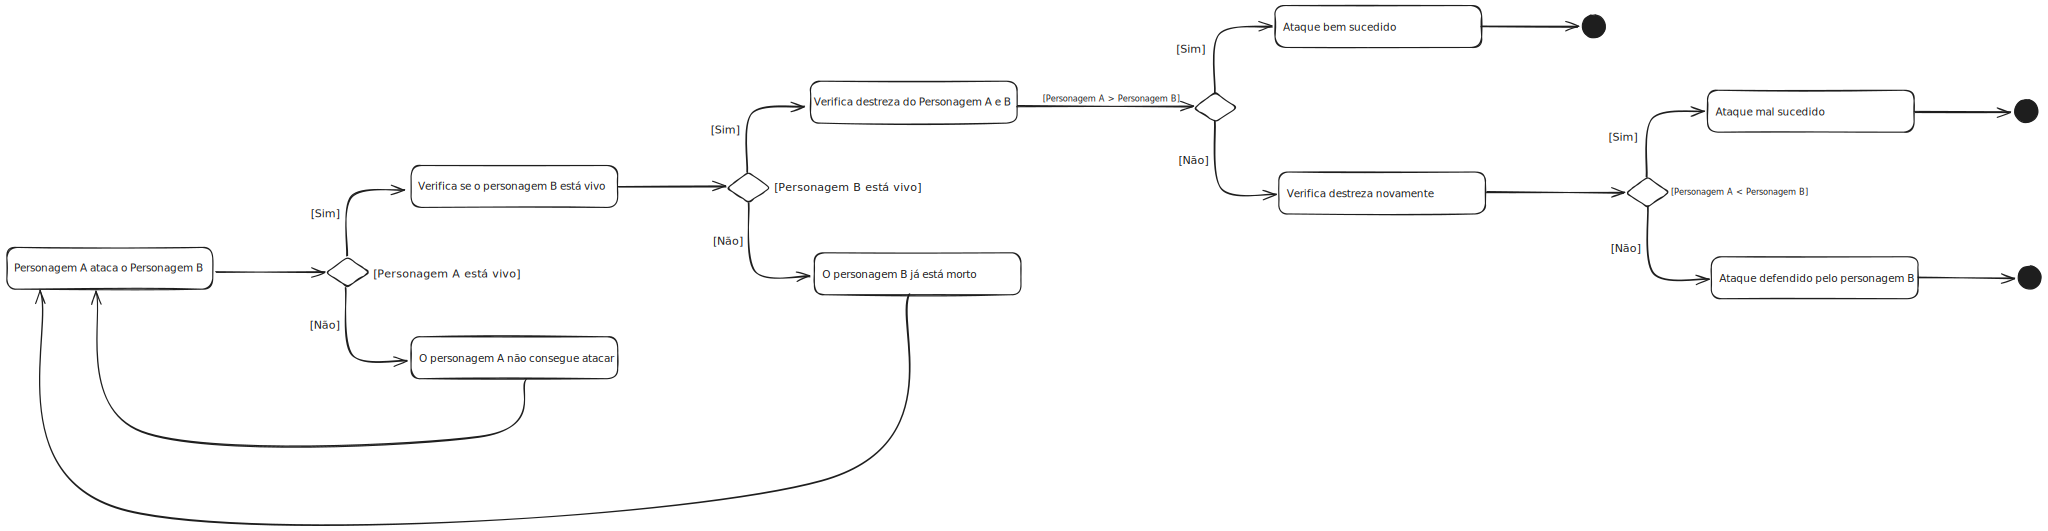
\includegraphics[width=\textwidth]{ilustracaoLPOO.png}
    \label{fig:exemplo}
\end{figure}

O segundo aspecto foi em relação às casas decimais, que estavam aparecendo com vírgula ao invés de ponto. Além disso, em um certo momento, as casas decimais estavam sendo exibidas de maneira errada, com muitos números após a vírgula.

Outro aspecto foi a demora para entender os status. Eu estava implementando incorretamente a parte responsável pela exibição da saída, o que resultava em algumas saídas invertidas, até notar que o status sempre é impresso inicialmente pelo status de quem está atacando.

\begin{lstlisting}[language=Java, caption={Implementação Antes de Corrigir}]
personagens[0].printStatus();
personagens[1].printStatus();
// Mago [Morto, Forca: 10.0, Destreza: 5.0, Magia da Transmutação]
// Mago [Saude: 10.0, Forca: 10.0, Destreza: 6.0, Psi-kappa]
\end{lstlisting}

\begin{lstlisting}[language=Java, caption={Implementação Após de Corrigir}]
personagens[ataque - 1].printStatus();
personagens[defesa - 1].printStatus();
// Mago [Saude: 10.0, Forca: 10.0, Destreza: 6.0, Psi-kappa]
// Mago [Morto, Forca: 10.0, Destreza: 5.0, Magia da Transmutação]
\end{lstlisting}

\vspace{1.5cm}
\Large \textbf{5. Soluções}

\justifying
Decidi agrupar as soluções, juntamente com os esclarecimentos e comentários, na seção anterior.

\end{document}